\documentclass[12pt,a4paper]{article}
\usepackage{pgf}
% \usepackage[condensed,math]{kurier}
% \usepackage[T1]{fontenc}
\usepackage{svg}
\usepackage{tikz}
\usepackage{stanli}
\usepackage{afterpage}
\usepackage{multirow}
\usepackage{subfig}
\usepackage{pgfpages}
\usepackage{svg}
\usepackage{rotating}

%\usepackage{times}


\pgfpagesdeclarelayout{boxed}
{
	\edef\pgfpageoptionborder{0pt}
}
{
	\pgfpagesphysicalpageoptions
	{%
		logical pages=1,%
	}
	\pgfpageslogicalpageoptions{1}
	{
		border code=\pgfsetlinewidth{2pt}\pgfstroke,%
		border shrink=\pgfpageoptionborder,%
		resized width=.9\pgfphysicalwidth,%
		resized height=.9\pgfphysicalheight,%
		center=\pgfpoint{.5\pgfphysicalwidth}{.5\pgfphysicalheight}%
	}%
}

\pgfpagesuselayout{boxed}


% Language setting
% Replace `english' with e.g. `spanish' to change the document language
\usepackage[english]{babel}

% Set page size and margins
% Replace `letterpaper' with `a4paper' for UK/EU standard size
\usepackage[a4paper,top=2cm,bottom=1.5cm,left=1.5cm,right=1.5cm,marginparwidth=1.75cm]{geometry}

% Useful packages
\usepackage{amsmath}
\usepackage{graphicx}
\usepackage[colorlinks=true, allcolors=blue]{hyperref}

\title{}
\author{}
\date{}

\begin{document}
	
	\newcommand{\subf}[2]{%
		{\small\begin{tabular}[t]{@{}c@{}}
				#1\\#2
		\end{tabular}}%
	}
	
	\begin{titlepage}
		\begin{center}
			
			\textbf{}
            
\includegraphics[width=1\textwidth]{utt.png}

            \vspace*{3cm}

			\vspace{1.5cm}
			
			\Huge
			\textbf{Introduction to service workers}
			
			\vspace{0.8cm}
			\large
			
			\vspace{0.5cm}
			\LARGE
			
			
			\vfill
			
			
			
			\vspace{0.8cm}
			
			
			
			\Large
			
			
			
			
		\end{center}
		\Large
		\begin{tabbing}
			\hspace*{1em}\= \hspace*{8em} \= \kill % set the tabbings
			\> Name:\>  \textbf{López Bautista Cristian Alexis} \\
			\> Group:\>  10-B \\
			\> Subject:\>  Progressive Web Applications  \\
			\> Professor:  \> Dr. Ray Brunet Parra Galaviz \\
			\> Date: \>  Wednesday, February 28th, 2024
		\end{tabbing}
		
	\end{titlepage}
	
	
	
	\section{Introduction}

    \paragraph{Service workers are a vital component of modern web development, offering
    powerful capabilities to enhance web applications with offline functionality, background
    synchronization, and push notifications. Essentially, they are scripts that run in the
    background of a web page, independent of the main browser thread. This enables
    them to intercept network requests, cache resources, and manage offline content,
    providing users with a seamless experience even in low-connectivity environments.
    By leveraging service workers, developers can create web apps that feel more like
    native applications, improving user engagement and overall satisfaction.}

    \paragraph{In addition to offline capabilities, service workers enable efficient caching
    strategies, allowing web applications to load faster and perform better, especially on
    repeat visits. With the ability to update themselves independently of the main
    application, service workers ensure that users always have the latest version of the
    web app, reducing reliance on traditional update mechanisms. Furthermore, service
    workers can handle background tasks such as periodic data synchronization, enabling
    real-time updates and notifications even when the web page is not actively being
    viewed. Overall, service workers represent a powerful tool for building robust,
    responsive web applications that excel in both online and offline scenarios.}

    \clearpage
    
    \section{What is a service worker?}

    \paragraph{A Service Worker is a type of web worker that runs in the background of a web
    application, independent of the web page’s main thread. They allow developers to
    build offline web applications, load faster, and provide a more reliable user experience.
    Service Workers are compatible with plain vanilla JavaScript applications, React,
    Angular, Svelte, Vue, etc.}

    \paragraph{Service workers essentially act as proxy servers that sit between web
    applications, the browser, and the network (when available). They are intended,
    among other things, to enable the creation of effective offline experiences, intercept
    network requests and take appropriate action based on whether the network is
    available, and update assets residing on the server. They will also allow access to
    push notifications and background sync APIs.}

    \paragraph{Web applications can become more responsive and reliable by using Service
    Workers, even in challenging network conditions. They can also provide a seamless
    experience to users, regardless of whether they are online or offline, which can lead
    to higher user engagement and satisfaction.}

    \begin{figure}[h!]
      \centering
      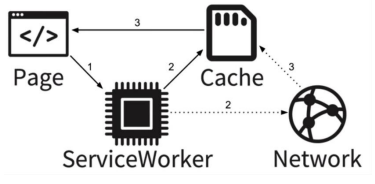
\includegraphics[width=0.5\textwidth]{diagram.png}
      \caption{Service worker diagram.}
    \end{figure}

    \section{The premise of Service Workers}

    \paragraph{One overriding problem that web users have suffered with for years is loss of
    connectivity. The best web app in the world will provide a terrible user experience if
    you can't download it. There have been various attempts to create technologies to
    solve this problem, and some of the issues have been solved. But the overriding
    problem is that there wasn't a good overall control mechanism for asset caching and
    custom network requests.}
    
    \paragraph{Service workers fix these issues. Using a service worker you can set an app up
    to use cached assets first, thus providing a default experience even when offline,
    before then getting more data from the network (commonly known as "offline first").}
    
    \paragraph{This is already available with native apps, which is one of the main reasons native
    apps are often chosen over web apps.}

    \section{How does a Service Worker work?}

    \paragraph{A service worker is an event-driven worker registered against an origin and a
    path. It takes the form of a JavaScript file that can control the webpage/site that it is
    associated with, intercepting, and modifying navigation and resource requests, and
    caching resources in a very granular fashion to give you complete control over how
    your app behaves in certain situations (the most obvious one being when the network
    is not available).}
    
    \paragraph{A service worker is run in a worker context: it therefore has no DOM access and runs on a different thread to the main JavaScript that powers your app, so it is non-blocking.
    It is designed to be fully async; as a consequence, APIs such as synchronous XHR
    and Web Storage can't be used inside a service worker.}
    
    \paragraph{Service workers can't import JavaScript module dynamically, and import() will throw if it is called in a service worker global scope. Static import using the import statement is allowed.}
    
    \paragraph{Service workers only run over HTTPS, for security reasons. Most significantly, HTTP
    connections are susceptible to malicious code injection by man in the middle attacks,
    and such attacks could be worse if allowed access to these powerful APIs. In Firefox,
    service worker APIs are also hidden and cannot be used when the user is in private
    browsing mode.}

    \begin{figure}[h!]
      \centering
      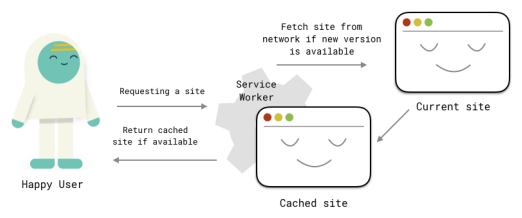
\includegraphics[width=0.5\textwidth]{cache.png}
      \caption{Service worker diagram.}
    \end{figure}

    \section{Setting up a Service Worker}

    \paragraph{Service workers are enabled by default in all modern browsers. To run code
    using service workers, you'll need to serve your code via HTTPS — Service workers
    are restricted to running across HTTPS for security reasons. A server supporting
    HTTPS is necessary. To host experiments, you can use a service such as GitHub,
    Netlify, Vercel, etc. In order to facilitate local development, localhost is considered a
    secure origin by browsers as well.}

    \clearpage

    \section{Conclusion}

    \paragraph{In conclusion, service workers play a pivotal role in shaping the future of web
    development by bridging the gap between web and native applications. With their
    ability to provide offline functionality, efficient caching, and background
    synchronization, service workers empower developers to create web applications that
    rival the performance and user experience of their native counterparts. By embracing
    service workers, developers can deliver fast, reliable, and engaging web experiences
    that adapt seamlessly to varying network conditions. As the web continues to evolve,
    service workers will remain a cornerstone technology, driving innovation and pushing
    the boundaries of what's possible on the modern web.}

    \clearpage

	\section{Bibliography}

    \begin{enumerate}
    
      \item MDN Contributors. (2023, july 7th). Using Service Workers. MDN Web Docs.
      February 28th, 2024,
      
    \href{https://developer.mozilla.org/enUS/docs/Web/API/Service_Worker_API/Using_Service_Workers}{https://developer.mozilla.org/enUS/docs/Web/API/Service_Worker_API/Using_Service_Workers}

      \item MDN Contributors. (2024, february 8th). Service Worker API - Web APIs. MDN
        Web Docs. February 28th, 2024,
        
      \href{https://developer.mozilla.org/en-US/docs/Web/API/Service_Worker_API}{https://developer.mozilla.org/en-US/docs/Web/API/Service_Worker_API}

      \item Vargas, P. (2023, 22 junio). Intro to JavaScript Service Workers - the PayPal Technology blog - medium. Medium.
      
      \href{https://medium.com/paypal-tech/intro-to-javascript-service-workers-43298c365549}{https://medium.com/paypal-tech/intro-to-javascript-service-workers-43298c365549}
      
    \end{enumerate}
	
	
\end{document}